\documentclass[18pt,handout]{beamer}

\usepackage{skript}
\setbeamertemplate{theorems}[numbered]


\title[Einfache Wurzeln]{Endliche Spiegelungsgruppen:\\
Einfache Wurzeln}
\author{Pavel Zwerschke}
\date{17. Juni 2019}
\titlegraphic{
\includegraphics[scale=0.3]{kitlogo_de_rgb.pdf}}

\usetheme{Berlin}

\begin{document}

\begin{frame}
    \maketitle
\end{frame}

\begin{frame}
    \tableofcontents
\end{frame}

\section{Wiederholungen Wurzeln}

\begin{frame}{Wurzel}
    Spiegelung an Hyperebene \( \mathscr{P} \) 
    lässt sich durch einen Vektor
    \( 0 \neq r \in \mathscr{P}^{\bot} \)
    beschreiben:
    \[ s_r(x) = x 
    - 2\frac{\scalarprod{x}{r}}{\scalarprod{r}{r}} r \]
    \pause
    
    Es gilt \( \forall x \in \mathscr{P}: s_r(x) = x \) 
    und \( s_r(r) = -r \). \pause

    Da Basis \( B \subset \mathscr{P} \cup \set{r} \) 
    existiert, folgt aus linearer Fortsetzung, dass 
    \( s_r \) Spiegelung an \( \mathscr{P} \) darstellt.

    \pause
    Außerdem gilt \( s_r^2 = 1 \).

    \( \Rightarrow \pm r \) sind Wurzeln von \( s_r \).

    \( \Delta = \set{ r \;\vert\; r \text{ ist Wurzel} } \) 
    nennen wir Wurzelsystem.
\end{frame}
\section{Positive und einfache Wurzeln}
\begin{frame}{Problem mit Wurzelsystemen}
    Problem: \( \Delta \) kann sehr groß werden. \pause

    Lösungsansatz: Suchen nach linear unabhängigen 
    Untermengen von \( \Delta \), mit denen \( \Delta \)
    konstruiert werden kann.
\end{frame}

\begin{frame}{\( \Delta_t^+ \) und \( \Delta_t^- \)}
    Sei \( t \in V \) so, dass \( \scalarprod{t}{r} \neq 0 
    \; \forall r \in \Delta \).\pause

    \( \Delta \) lässt sich in zwei Teilmengen 
    \( \Delta_t^+ = 
    \set{r \in \Delta \;\vert \; \scalarprod{t}{r} > 0} \) 
    und \( \Delta_t^- = 
    \set{r \in \Delta \;\vert \; \scalarprod{t}{r} < 0} \) 
    aufteilen. \pause
    % geometrisch gesehen liegen Delta^+ und Delta^- 
    % auf unterschiedlichen Hyperebenen von 
    % t^\bot

    Sei \( r \in \Delta \). \( \Rightarrow -r \in \Delta \), 
    da \( \scalarprod{t}{-r} = -\scalarprod{t}{r} \).\\
    \( \Rightarrow r \) und \( -r \) sind in 
    gegensätzlichen Mengen. \pause
    \[ \Rightarrow \abs{\Delta_t^+} = \abs{\Delta_t^-}. \]
\end{frame}

\section{Einfache Wurzelsysteme}
\begin{frame}{Definition \( t \)-Basis}
    \( \Pi \subset \Delta_t^+ \) heißt \( t \)-Basis, 
    wenn gilt:
    \begin{itemize}
        \item Jedes \( r \in \Delta_t^+ \) ist 
        eine Linearkombination mit ausschließlich 
        nichtnegativen Koeffizienten.
        \item \( \Pi \) ist minimal.
    \end{itemize} \pause
    Es existiert mindestens eine \( t \)-Basis, 
    da \( \Delta \) endlich ist. \pause
    
    Da \( \Delta_t^+ = - \Delta_t^- \), ist jedes 
    \( r \in \Delta_t^- \) eine Linearkombination 
    mit ausschließlich nichtpositiven Koeffizienten.

    \pause
    Wird noch gezeigt: \( \Pi \) ist eine Basis.
\end{frame}

\begin{frame}{Definition \(t\)-positiv, \( t \)-negativ}
    \( x \in V \) heißt \(t\)-positiv, wenn 
    die Linearkombination von \(x\) zur 
    Basis ausschließlich nichtnegativ ist.

    Analog für \( t \)-negativ.
    % Hängt nicht von \( \Pi \) ab, da \( \Pi \) 
    % eindeutig.
\end{frame}

\begin{frame}
    \begin{satz} % Proposition 4.1.4
        % satz 1
        % nicht unbedingt beweisen
        Seien \( r_i, r_j \in \Pi, i \neq j \) und 
        \( \lambda_i, \lambda_j \in \R_+ \). 
        Der Vektor \( x = \lambda_i r_i - \lambda_j r_j \) 
        ist weder \( t \)-positiv noch \( t \)-negativ.
    \end{satz}
\end{frame}

\begin{frame}
    \begin{bew}
        Wenn \(x\) positiv wäre, könnten 
        wir schreiben 
        \[ x = \lambda_i r_i - \lambda_j r_j 
        = \sum_{k=1}^m \mu_k r_k \]
        mit allen \( \mu_i \geq 0 \). \pause

        Fall 1 \( \lambda_i \leq \mu_i \):
        \[ \Leftrightarrow 0 
        = - \lambda_i r_i + \lambda_j r_j 
        + \sum_{k=1}^m \mu_k r_k \]
        
        \renewcommand{\qedsymbol}{}
    \end{bew}
\end{frame}

\begin{frame}
    \begin{bew}
        \[ \Leftrightarrow 0 = (\mu_i - \lambda_i)
        r_i + (\mu_j + \lambda_j) 
        r_j + 
        \sum_{
            \substack{k \in \set{1,\ldots, m}\\k \neq i,j}}
        \mu_k r_k. \] \pause
        Dauraus folgt 
        \[ 0 = \scalarprod{t}{ 
            (\mu_i - \lambda_i) r_i + (\mu_j + \lambda_j) r_j 
        + \sum_{\substack{k \in \set{1,\ldots, m}\\k \neq i,j}}
        \mu_k r_k
        } \geq \lambda_j \scalarprod{t}{r_j} > 0. 
        \text{ \Lightning} \]

        \renewcommand{\qedsymbol}{}
    \end{bew}
\end{frame}

\begin{frame}
    \begin{bew}
        Fall 2: \( \lambda_i > \mu_i \): 
        \[ (\lambda_i - \mu_i) r_i
        = (\mu_j + \lambda_j) r_j 
        + \sum_{\substack{k \in \set{1,\ldots, m}\\k \neq i,j}}
        \mu_k r_k. \]
        Dann ließe sich \( r_i \) als eine 
        nichtnegative Linearkombination von 
        \( \Pi \setminus \set{r_i} \) darstellen. 
        \Lightning{} zur Minimalität von 
        \( \Pi \).

        Wenn \( x \) negativ ist, müsste \( -x \) 
        positiv sein, was nicht möglich ist.
    \end{bew}
\end{frame}

\begin{frame}
    % satz 2
    \begin{satz} % Proposition 4.1.5
        % beweis so kurz, kann man kurz anschreiben
        Seien \( r_i, r_j \in \Pi, i \neq j \), es 
        sei \( S_i \) die Spiegelung an \( r_i \). 

        Dann ist \( S_i r_i \in \Delta_t^+ \) und 
        \( \scalarprod{r_i}{r_j} \leq 0 \).
    \end{satz}
    \pause
    \begin{bew}
        Da \( S_i r_j \in \Delta \), ist \( S_i r_j \) 
        entweder positiv oder negativ. Da 
        \[ S_i r_j = r_j - 2 \scalarprod{r_j}{r_i} r_i, \]
        mit \( \lambda_j = 1 \), muss 
        \( \lambda_i \geq 0 \), da sonst 
        \( S_i r_i \notin \Delta \). \pause

        \( \Rightarrow \scalarprod{r_i}{r_j} \leq 0 
        \Rightarrow S_i r_j \) 
        positiv.
    \end{bew}
    % geometrische Bedeutung:
    % <r_i, r_j> \leq 0 bedeutet, dass Winkel zwischen 
    % r_i und r_j stumpf ist, da skalarprod der cosinus vom winkel 
    % ist.
\end{frame}

\begin{frame}
    % satz 3
    \begin{satz} % Proposition 1.4.6
        % beweis mittels bild?
        Seien \( x_1, \ldots, x_m \in V \) alle auf derselben 
        Seite einer Hyperebene \( \mathscr{P} \). \\
        Falls \( \scalarprod{x_i}{x_j} \leq 0 \) immer wenn 
        \( i \neq j \), dann ist \( \set{x_1, \ldots, x_m} \) 
        linear unabhängig.
    \end{satz} \pause

    \begin{bew}
        Wenn das der Fall wäre, dann gäbe es 
        \( \lambda_i, \mu_i \geq 0 \) mit 
        manchen \( \lambda_i > 0 \), sodass 
        \[ \sum_{i=1}^k \lambda_i x_i 
        = \sum_{i=k+1}^m \mu_i x_i. \]

        \renewcommand{\qedsymbol}{}
    \end{bew}
\end{frame}

\begin{frame}
    \begin{bew}
        Dann gilt 
        \begin{align*}
            \onslide<1->{0 \leq \norm{\sum_{i=1}^k \lambda_i x_i}^2 
            &= \scalarprod{\sum_{i=1}^{k} \lambda_{i} x_{i}}{
            \sum_{j=1}^{k} \lambda_{j} x_{j}} \\}
            \onslide<2->{
                &= \scalarprod{\sum_{i=1}^{k} \lambda_{i} x_{i}}{
                \sum_{j=k+1}^{m} \mu_{j} x_{j}} \\
            }
            \onslide<3>{
                &= \sum_{i=1}^{k} \sum_{j=k+1}^{m} \lambda_{i} \mu_{j}
                \scalarprod{x_i}{x_j} 
                \leq 0. % nach Voraussetzung
            }
        \end{align*}
        
        \renewcommand{\qedsymbol}{}
    \end{bew}
\end{frame}
\begin{frame}
    \begin{bew}
        Es gilt jedoch nun 
        \[ 0 = \scalarprod{\sum_{i=1}^{k} \lambda_i x_i}{x} 
        = \sum_{i=1}^k \lambda_i \scalarprod{x_i}{x} > 0. \text{ \Lightning{}} \]
        % da manche lambda_i > 0
        \pause
        Deshalb muss \( \set{x_1, \ldots, x_m} \) linear 
        unabhängig sein.
    \end{bew}
\end{frame}

\begin{frame}
    % Satz 4
    \begin{satz} % Theorem 1.4.7
        % beweis anschreiben
        Sei \( \Pi \) eine \(t\)-Basis von \( \Delta \). Dann ist 
        \( \Pi \) eine Basis für \( V \).
    \end{satz}
    \pause
    \begin{bew}
        \begin{itemize}
            \item \( \Delta \) erzeugt \( V \). (s. Vortrag \gqq{Wurzelsysteme})\\
            Da jedes \( r \in \Delta \) eine Linearkombination von \( \Pi \) ist, 
            ist \( \Pi \) Erzeugendensystem. \pause
            \item<2-> \( \Delta \) ist nach Satz 2 und 3 linear unabhängig.
        \end{itemize} \pause
        \( \Rightarrow \Pi \) ist eine Basis von \(V\).
    \end{bew}
\end{frame}

\begin{frame}
    % Satz 5
    \begin{satz} % Proposition 4.1.8
        % beweis anschreiben
        Es gibt nur eine \( t \)-Basis von \( \Delta \).
    \end{satz}
\end{frame}

\section{Beispiele}
\begin{frame}{Beispiele}
    Sei \( \mathscr{G} = \mathscr{H}_2^4 \), 
    die vier Spiegelungen in \( \mathscr{G} \) 
    generieren es.
    \[ \Delta = \set{ \pm(1,0), \pm(0,1), (\pm 1, \pm 1) }. \]
    \onslide<2->{Wähle \( t = 2( \cos(\frac{3\pi}{8}), \sin(\frac{3\pi}{8}) ) \).}

    \begin{columns}[c]
        \begin{column}{0.7\textwidth}
            \begin{align*}
                \onslide<3->{\Rightarrow \Delta_+ 
                &= \set{(1,0), (1,1), (0,1), (-1,1)}, \\}
                \onslide<4->{\Pi &= \set{ (1,0), (-1,1) }.}
            \end{align*}
        \end{column}
        \begin{column}{0.3\textwidth}
         \begin{figure}
            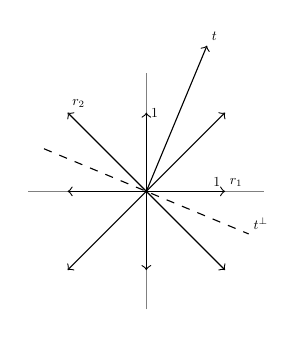
\begin{tikzpicture}
                \draw[thin, gray] (-1.5,0) -- (1.5,0);
                \draw[thin, gray] (0,-1.5) -- (0,1.5);
                \draw[->] (0,0) -- (0,1) node[right, scale=0.5] {\( 1 \)};
                \draw[->] (0,0) -- (0,-1);
                \draw[->] (0,0) -- (-1,0);
                \draw[->] (0,0) -- (1,0) node[above left, scale=0.5] {\( 1 \)};
                \onslide<4->{\draw (1,0) node[above right, scale=0.5] {\( r_1 \)};}
                \draw[->] (0,0) -- (-1, 1);
                \onslide<4->{\draw (-1, 1) node[above right, scale=0.5] {\( r_2 \)};}
                \draw[->] (0,0) -- (-1,-1);
                \draw[->] (0,0) -- (1,1);
                \draw[->] (0,0) -- (1,-1);
                \onslide<2->{\draw[->] (0,0) -- (0.77, 1.85) node[above right, scale=0.5] {\( t \)};}
                \onslide<2->{\draw[dashed] (-1.3,-0.77 / 1.85 * -1.3) -- (1.3, -0.77 / 1.85 * 1.3) 
                node[above right, scale=0.5] {\( t^\bot \)};}
            \end{tikzpicture}
          \end{figure}
        \end{column}
      \end{columns}
\end{frame}

\section{Spiegelungsgruppen generieren}
\begin{frame}
    % Satz 6
    \begin{satz} % Proposition 4.1.9
        % nicht unbedingt beweisen
        Sei \( S_i \) die Spiegelung an 
        \( r_i \in \Pi = \set{r_1, \ldots, r_n} \).
        Wenn \( r \in \Delta^+ \) und \( r_i \neq r \), 
        dann gilt \( S_i r \in \Delta^+ \).
    \end{satz}
    \pause
 %   % Satz 7
%    \begin{satz} % Proposition 4.1.10
  %      % gar nicht
 %       Sei \( x \in V\). Dann gibt es ein \( T \in 
 %       \mathscr{G}_t := \langle 
  %      \set{S_i \;\vert\; r_i \in \Pi} \rangle \) so, dass
   %     \( \scalarprod{Tx}{r_i} \geq 0 \;\forall r_i \in \Pi \).
  %  \end{satz}
\end{frame}

\begin{frame}
    % Satz 7
    \begin{satz} % Proposition 4.1.11
        % nicht so interessant, nur satz hinschreiben
        Sei \( r \in \Delta^+ \). Es existiert ein \( T \in 
        \mathscr{G}_t \) so, dass 
        \( Tr \in \Pi \).
    \end{satz}
\end{frame}

\begin{frame}
    % Satz 8
    \begin{satz} % Theorem 4.1.12
        % wichtiger, beweisen
        Die einfachen Spiegelungen \( S_1, \ldots, S_n \) 
        erzeugen \( \mathscr{G} \).
    \end{satz}
    \pause
    \begin{bew}
        Da \( \mathscr{G} = \langle S_r \;\vert\; r \in \Delta \rangle \) 
        und \( S_{-r} = S_r \), genügt es, zu zeigen, dass wenn 
        \( r\in \Delta^+ \), dann \( S_r \in \mathscr{G}_t \).

        \pause
        Sei \( r \in \Delta^+ \). Nach Satz 7 gibt es 
        ein \( T \in \mathscr{G}_t \), sodass 
        \( r_i := Tr \in \Pi \).

        \pause
        Es gilt:
        \[ S_r = T^{-1} S_i T \in \mathscr{G}_t. \]
        \[ \Rightarrow \mathscr{G} \subset \mathscr{G}_t. \]
        \[ \Rightarrow \mathscr{G} = \mathscr{G}_t. \]
    \end{bew}
\end{frame}

\begin{frame}{Abschluss}
    Für jede endliche Spiegelungsgruppe 
    \( \mathscr{G} \) existiert eine Basis 
    einfache \( t \)-Basis \( \Pi \) 
    von \( V \). 
    \pause
    
    Die Spiegelungen in 
    \( \Pi \) erzeugen \( \mathscr{G} \).
\end{frame}

\end{document}